\chapter{BPMN Python}
\label{cha:bpmn-python}
\section{Project description}
The \emph{bpmn\_python} package provide means to represent BPMN diagram as an object during program execution. The main functionalities of this package is an import and export of BPMN diagram from XML files (compatible with official BPMN 2.0 XML Schema). Handling thee spreadsheet-based model descriptions is still in early stage of development, but it is able to work with basic examples. In addition, this library provides methods to manually create a simple BPMN process by making a Python script and also implements a set of diagram complexity metrics from article~\cite{kluza-metrics}.
\section{Manual generation of BPMN diagram}
This section shows a simple example of how to create a BPMN diagram using \emph{bpmn\_python}. This example is taken form package wiki\footnote{\url{https://github.com/KrzyHonk/bpmn-python/wiki}}. Current version of \emph{bpmn\_python} allows the user to add basic BPMN elemenst, such as start, stop events, tasks, collapsed sub-processes or gateways (inclusive, exclusive, parallel) to BPMN diagram.\\
Firs, it is required to import the script with \texttt{\emph{BPMNDiagramGraph}} class:
\begin{lstlisting}[language=python]
import bpmn_python.bpmn_diagram_rep as diagram
\end{lstlisting}
Then, we can create a BPMNDiagramGraph object:
\begin{lstlisting}[language=python]
bpmn_graph = diagram.BPMNDiagramGraph()
bpmn_graph.create_new_diagram_graph(diagram_name="diagram1")
\end{lstlisting}
Using \texttt{\emph{add\_start\_event\_to\_diagram}} and \texttt{\emph{add\_task\_to\_diagram}}, we can create a new start event and task. Then, we have to connect those elements with sequence flow.\\
User is allowed to change few attributes of new elements - for each element created in this example a name will be given (by default name is an empty string).\\
Notice that all of the methods used to add new elements into diagram returns two objects - a string representing an ID of a new element and a reference to object representing this element. Since this example requires only an ID of element, we skip the object reference using anonymous variable (denoted by \_).
\begin{lstlisting}[language=python]
[start_id, _] = bpmn_graph.add_start_event_to_diagram(start_event_name="start_event")
[task1_id, _] = bpmn_graph.add_task_to_diagram(task_name="task1")
bpmn_graph.add_sequence_flow_to_diagram(start_id, task1_id, "start_to_one")
\end{lstlisting}
Now we can create an exclusive gateway (fork and join element) with two tasks:
\begin{lstlisting}[language=python]
[exclusive_gate_fork_id, _] = bpmn_graph.add_exclusive_gateway_to_diagram(gateway_name="exclusive_gate_fork")
[task1_ex_id, _] = bpmn_graph.add_task_to_diagram(task_name="task1_ex")
[task2_ex_id, _] = bpmn_graph.add_task_to_diagram(task_name="task2_ex")
[exclusive_gate_join_id, _] = bpmn_graph.add_exclusive_gateway_to_diagram(gateway_name="exclusive_gate_join")

bpmn_graph.add_sequence_flow_to_diagram(task1_id, exclusive_gate_fork_id, "one_to_ex_fork")
bpmn_graph.add_sequence_flow_to_diagram(exclusive_gate_fork_id, task1_ex_id, "ex_fork_to_ex_one")
bpmn_graph.add_sequence_flow_to_diagram(exclusive_gate_fork_id, task2_ex_id, "ex_fork_to_ex_two")
bpmn_graph.add_sequence_flow_to_diagram(task1_ex_id, exclusive_gate_join_id, "ex_one_to_ex_join")
bpmn_graph.add_sequence_flow_to_diagram(task2_ex_id, exclusive_gate_join_id, "ex_two_to_ex_join")
\end{lstlisting}

And finally, add second task and end event:
\begin{lstlisting}[language=python]
[task2_id, _] = bpmn_graph.add_task_to_diagram(task_name="task2")
[end_id, _] = bpmn_graph.add_end_event_to_diagram(end_event_name="end_event")
bpmn_graph.add_sequence_flow_to_diagram(exclusive_gate_join_id, task2_id, "ex_join_to_two")
bpmn_graph.add_sequence_flow_to_diagram(task2_id, end_id, "two_to_end")
\end{lstlisting}
Figure~\ref{fig:manual_gen_example} presents a visualization of created BPMN diagram.
\begin{figure}[H]
	\centering
	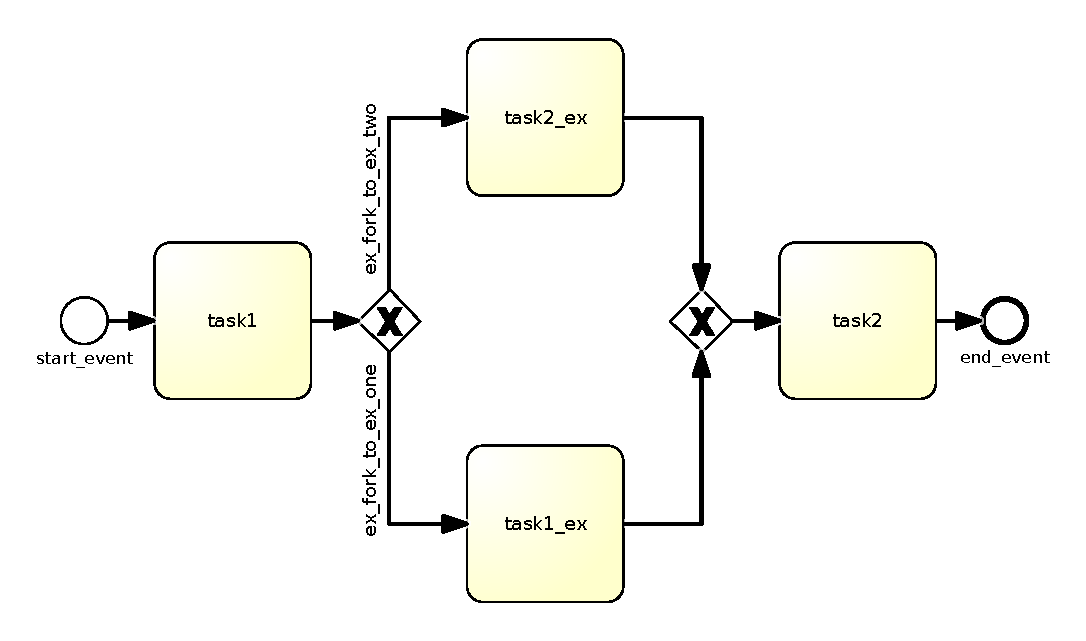
\includegraphics[scale=0.6]{./images/manually_gen_example.pdf}
	\caption{BPMN diagram manually created using \emph{bpmn\_python} package}
	\label{fig:manual_gen_example}
\end{figure}

